%%%%%%%%%%%%%%%%%%%% fe_springer.tex %%%%%%%%%%%%%%%%%%%%%%%%%%%%%%%%%%
%
% Financial Engineering and the Evidence -- Springer (svmult) layout,
% following springer_agentic.tex. Converted from the Beautybook version.
%
%%%%%%%%%%%%%%%%%%%%%%%%%%%%%%%%%%%%%%%%%%%%%%%%%%%%%%%%%%%%%%%%%%%%%%%

\documentclass[graybox,openany]{style/svmult}
\usepackage[paperwidth=7.5in, paperheight=9.25in, top=2.5cm, bottom=2.5cm,
            left=2.5cm, right=2.5cm]{geometry}

% ----------------------------------------------------------------------
% Fonts and encoding (as in springer_agentic.tex)
% ----------------------------------------------------------------------
\usepackage[utf8]{inputenc}
\usepackage[T1]{fontenc}
\usepackage{type1cm}
\usepackage{newtxtext}
\usepackage{newtxmath}       % Times Roman text and math
\usepackage{bm}

% ----------------------------------------------------------------------
% General packages
% ----------------------------------------------------------------------
\usepackage{amsmath}         % \eqref, equation environments
\usepackage{graphicx}
\usepackage{xcolor}
\usepackage{pdfpages}        % chapter infographics, cover
\usepackage{booktabs}
\usepackage{array}
\usepackage{tabularx}
\usepackage{longtable}
\usepackage{multicol}
\usepackage[bottom]{footmisc}
\usepackage{enumitem}
\setlist[itemize]{itemsep=0pt}
\setlist[enumerate]{itemsep=0pt}
\usepackage{url}
\pagecolor{white}

% ----------------------------------------------------------------------
% Layout (as in springer_agentic.tex)
% ----------------------------------------------------------------------
\usepackage{tocloft}
\setlength{\parskip}{0.5em}
\usepackage{setspace} \setstretch{1.1}
\usepackage{chngcntr}
\counterwithin{section}{chapter}
\counterwithin{figure}{chapter}
\usepackage[justification=centering]{caption}
\setlength{\abovecaptionskip}{0pt}
\setlength{\belowcaptionskip}{0pt}
\usepackage{titlesec}
\titlespacing*{\section}{0pt}{*1.0}{*0.7}
\titlespacing*{\subsection}{0pt}{*1.0}{*0.7}
\titlespacing*{\subsubsection}{0pt}{*1.0}{*0.7}

\usepackage{fancyhdr}
\pagestyle{fancy}
\fancyhf{}
\fancyhead[C]{\thepage}
\fancyfoot[C]{\thepage}
\renewcommand{\headrulewidth}{0pt}

% ----------------------------------------------------------------------
% Figures drawn in TikZ / pgfplots (Chapters 3-7)
% ----------------------------------------------------------------------
\usepackage{pgfplots}
\pgfplotsset{compat=1.17}
\usepgfplotslibrary{fillbetween}
\usetikzlibrary{decorations.pathreplacing}

\definecolor{fenavy}{HTML}{1B2A6B}
\definecolor{fegray}{HTML}{4D4D4D}
\definecolor{feorange}{HTML}{B8481C}
\definecolor{feshade}{HTML}{F3F5FA}

% ----------------------------------------------------------------------
% Boxes
% ----------------------------------------------------------------------
\usepackage[most]{tcolorbox}   % breakable, skins (for borderline west)

% Callouts (What Failed, Lab at a glance, ...)
\newtcolorbox{callout}{%
  breakable, enhanced,
  colback=white, colframe=fenavy, boxrule=0.5pt, arc=1mm,
  borderline west={2.5pt}{0pt}{fenavy},
  left=8pt, right=8pt, top=4pt, bottom=4pt}

% Background box (was redefined in the Beautybook version)
\newenvironment{backgroundbox}[1]
{%
\begin{tcolorbox}[
    width=\textwidth, center,
    colback=gray!5, colframe=gray!70,
    enhanced, boxrule=0.5pt, breakable,
    left=0pt, right=5pt, top=4pt, bottom=4pt]
\linespread{1.1}\selectfont
\begin{list}{}{%
    \setlength{\labelwidth}{0.8cm}%
    \setlength{\labelsep}{0.25cm}%
    \setlength{\leftmargin}{1.05cm}%
    \setlength{\rightmargin}{0pt}%
    \setlength{\topsep}{0pt}%
    \setlength{\partopsep}{0pt}%
    \setlength{\parsep}{0pt}%
    \setlength{\itemsep}{0pt}%
    \setlength{\listparindent}{0pt}%
}
\item\relax
{\bfseries #1\par}\medskip
}
{%
\end{list}%
\end{tcolorbox}%
}

% ----------------------------------------------------------------------
% Theorem-like environments
% svmult already provides: theorem, lemma, corollary, proposition,
% definition, example, exercise, problem, remark, conjecture, ...
% The short Beautybook names are mapped onto them so chapters still compile.
% ----------------------------------------------------------------------
\newenvironment{defi}{\begin{definition}}{\end{definition}}
\newenvironment{thm}{\begin{theorem}}{\end{theorem}}
\newenvironment{lem}{\begin{lemma}}{\end{lemma}}
\newenvironment{prop}{\begin{proposition}}{\end{proposition}}
\newenvironment{exam}{\begin{example}}{\end{example}}
\newenvironment{cor}{\begin{corollary}}{\end{corollary}}

% ----------------------------------------------------------------------
% Q&A
% ----------------------------------------------------------------------
\newenvironment{qanda}
  {\begin{list}{}{\leftmargin=1cm \rightmargin=0cm \labelwidth=1cm
                  \labelsep=0.2cm \itemindent=0cm \parsep=0.2cm}}
  {\end{list}}
% svmult already defines \question, so clear both names first
\let\question\relax
\let\answer\relax
\newcommand{\question}[1]{\item[\textbf{Question:}] #1}
\newcommand{\answer}[1]{\item[\textbf{Answer:}] #1}

% ----------------------------------------------------------------------
% Code listings
% ----------------------------------------------------------------------
\usepackage{listings}
\lstset{
    basicstyle=\small\ttfamily,
    commentstyle=\color{gray!50!black!50},
    stringstyle=\rmfamily\color{red},
    keywordstyle=\normalfont\ttfamily,
    frame=leftline,
    framerule=0.5pt, rulecolor=\color{gray!80},
    numbers=left,
    numberstyle=\color{gray}\small,
    firstnumber=1, stepnumber=1, numbersep=8pt,
    showspaces=false, showstringspaces=false, keepspaces=true,
    showtabs=false, tabsize=2,
    captionpos=b, flexiblecolumns=true,
    breaklines=true, breakatwhitespace=false, breakautoindent=true,
    breakindent=1em,
    title=\lstname,
    escapeinside=``,
    xleftmargin=1em, xrightmargin=1em,
    aboveskip=1ex, belowskip=1ex,
    framextopmargin=1pt, framexbottommargin=1pt,
    abovecaptionskip=-2pt, belowcaptionskip=3pt,
    extendedchars=false, columns=flexible, mathescape=true,
    texcl=true, fontadjust
}

% ----------------------------------------------------------------------
% Index
% ----------------------------------------------------------------------
\usepackage{makeidx}
\makeindex             % run makeindex with the svind.ist style

% Load hyperref last
\usepackage[hidelinks]{hyperref}

%--------------------------------------------------------%
\begin{document}
%--------------------------------------------------------%

% Cover (optional; uncomment to include the front cover PDF)
%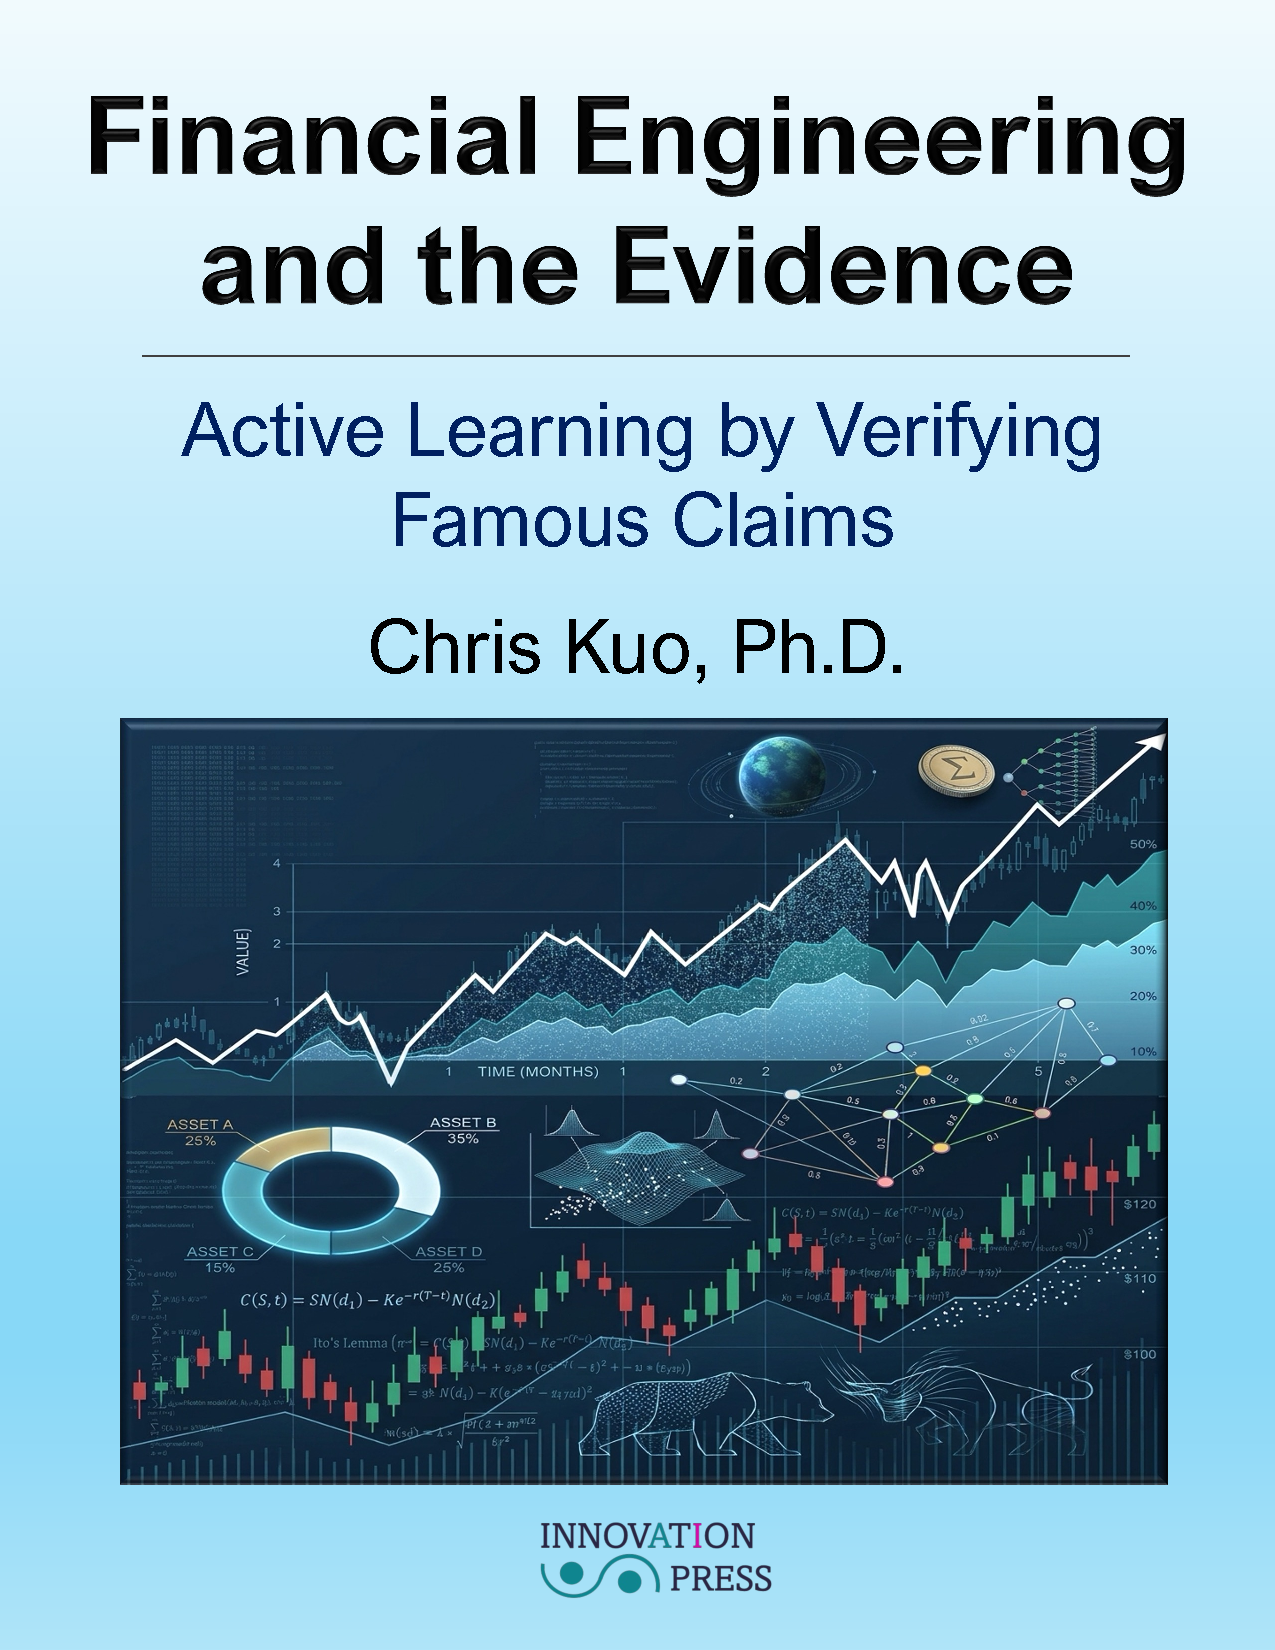
\includepdf{cover/The_frontcover_beautybook.pdf}

%------------------------ Publisher matter -------------------------%
\thispagestyle{empty}
\vspace*{\fill}
\footnotesize

\noindent Copyright \textcopyright{} Chris Kuo, Ph.D. \\
\\
\noindent All rights reserved. No part of this publication may be reproduced,
stored in a retrieval system, or transmitted in any form or by any means,
electronic, mechanical, photocopying, recording, scanning, or otherwise, except
as permitted under Section 107 or 108 of the 1976 United States Copyright Act,
without the prior written permission of the publisher, or in the case of brief
quotations embodied in critical reviews and certain other noncommercial uses
permitted by copyright law.

\noindent While every effort has been made to ensure the reliability of the
information presented in this publication, Innovation Press assumes no
responsibility for errors or omissions. However, neither the author nor
Innovation Press assumes any liability for damages resulting from the use of
the information contained herein. \\
\\
\noindent ISBN 979-8-9907810-8-5 \\
\\
\noindent First edition: January 2027 \\

\noindent This book was typeset using \LaTeX{} software. \\
\noindent The Innovation Press, \\
\noindent Ann Arbor, MI
\begin{figure}[!htbp]
  
\includegraphics[width=0.12\textwidth]{innovation_press.png}
\end{figure}

\vspace*{\fill}
\normalsize

\frontmatter

% -------------------------About the author------------------------------%
{
\thispagestyle{empty}
%\chapter*{About the Author}
%\addcontentsline{toc}{chapter}{About the Author}

\thispagestyle{empty}
\noindent{\LARGE\bfseries About the Author}\par
\vspace{1.5em}
\addcontentsline{toc}{chapter}{About the Author}   % delete if it shouldn't appear in the contents


\textbf{Chris Kuo} is an economist, data scientist and educator with more than 25 years of experience in quantitative modeling and analytics. 
His work centers on applied artificial intelligence, machine learning and data-driven decision making. He has led data science initiatives in enterprise environments
and is the inventor of a U.S.\ patent for data-driven analytical solutions.

In addition to his industry work, Chris teaches at Columbia University and has previously taught at Boston University, the University of New Hampshire and Liberty University, in economics, management and machine learning. He believes that students learn a method best when they are asked to verify a statement with it, especially in the age of AI. That belief is the philosophy behind this book.
He has published research in economics and management journals and is the author of ten books on applied AI, machine learning and analytics.

He holds a Ph.D. in Economics from Stony Brook University and a B.S. in Nuclear Engineering from National Tsing Hua University in Taiwan. He lives in New York City with his wife.

\medskip
\noindent His published books include (by year):

\begin{enumerate}[label=\arabic*., leftmargin=*, itemsep=0pt, topsep=4pt]
  \item \textbf{2027}\quad\textit{Financial Engineering and the Evidence: Active Learning by Verifying Famous Claims}
  \item \textbf{2026}\quad\textit{Agentic AI for Anomaly Detection: Building Your Own Agentic AI Systems Step by Step}
  \item \textbf{2026}\quad\textit{Modern Causal Inference: Methods and Applications: An Essential Hands-on Guide with DoWhy, EconML, CausalML, Causal-learn in Python}
  \item \textbf{2025}\quad\textit{Introduction to Statistics with Python: The Essential Guide to Data Analysis}
  \item \textbf{2024}\quad\textit{The Handbook of Anomaly Detection (2nd Edition): Cutting-edge Methods and Hands-On Code Examples}
  \item \textbf{2024}\quad\textit{Modern Time Series Forecasting Techniques For Predictive Analytics and Anomaly Detection: From Classical Foundations to Cutting-Edge Applications}
  \item \textbf{2023}\quad\textit{The Handbook of NLP with Gensim: Leverage topic modeling to uncover hidden patterns, themes, and valuable insights within textual data}
  \item \textbf{2023}\quad\textit{The Handbook of Anomaly Detection (1st Edition): Build and modernize your anomaly detection models with examples}
  \item \textbf{2022}\quad\textit{Transfer Learning for Image Classification: With Python examples}
  \item \textbf{2022}\quad\textit{The eXplainable A.I.: With Python Examples}
  \item \textbf{2021}\quad\textit{Modern Time Series Anomaly Detection: With Python and R examples}
\end{enumerate}

% ---- Dedication -------------------------------------------------------
%\cleardoublepage
\thispagestyle{empty}
\vspace*{\fill}
\vspace{2cm}
\begin{center}
  \textit{This book is dedicated to Nathan and Eileen,}\\[4pt]
  \textit{from Dad.}
\end{center}

\vspace{2cm}

\noindent\rule{\textwidth}{0.8pt}
\begin{center}
  \begin{minipage}{0.85\textwidth}
    \centering
    ``Trust in the \textsc{Lord} with all your heart and lean not on your own
    understanding; in all your ways submit to him, and he will make your
    paths straight.''\\[6pt]
    ---~Proverbs 3:5--6 (NIV)
  \end{minipage}
\end{center}
\noindent\rule{\textwidth}{0.8pt}

\vspace*{\fill}
}

%------------------------------TOC------------------------------------------%
\thispagestyle{empty}
\tableofcontents\let\cleardoublepage\clearpage

\mainmatter
\pagenumbering{arabic}

% ----------------------------Preface and Introduction-----------------%
\input{chapters/preface.tex}
\clearpage

%--------------------------- PART I ------------------------------------%
%\addcontentsline{toc}{chapter}{PART I: ...}
%\input{parts/part1_intro.tex}
% Chapter 1 -- Why Prices Are Hard to Predict, and Why Claims Need Testing
% Requires: amsmath, booktabs, array, tabularx, graphicx, tcolorbox (breakable, skins), hyperref or url.
% Defines the callout box only if the preamble has not.
\providecolor{fenavy}{HTML}{1B2A6B}
\providecolor{feshade}{HTML}{F3F5FA}
\makeatletter
\@ifundefined{callout}{%
  \newtcolorbox{callout}{breakable, enhanced,
    colback=white, colframe=gray!70, boxrule=0.5pt, arc=1mm,
    borderline west={2.5pt}{0pt}{gray!70},
    left=8pt, right=8pt, top=4pt, bottom=4pt}%
}{}
\makeatother

\chapter{Why Prices Are Hard to Predict, and Why Claims Need Testing}
\label{ch:01}

Every year, a great many investment strategies are presented with impressive track records. Fund reports show steady equity curves, academic papers report significant t-statistics, and online forums share backtests that turned \$10,000 into a fortune. Some of these strategies are genuinely good. The challenge, for anyone who wants to build or choose one, is to recognize which.

That is harder than it looks, because financial data make it unusually easy to find patterns that are not there. Returns are noisy, the history is short, and everyone searches the same data. Under those conditions, a strategy with no skill at all can look brilliant for a while, and a genuinely good strategy can look ordinary for a decade. But real skill leaves evidence that luck cannot fake for long, and this chapter shows how to read it.

The claim on trial in this chapter is the one every strategy builder hopes is true: \textbf{a long enough track record can reveal real skill.} Testing it means learning how long ``long enough'' is, and what else a record must show. The chapter then introduces the method the rest of the book uses: state the claim, understand it, verify it, judge it, and apply what survives.

By the end of the chapter you will be able to:

\begin{itemize}
  \item compute simple, log and excess returns, and convert monthly means and volatilities to annual ones;
  \item calculate a Sharpe ratio and judge whether a mean return is statistically different from zero;
  \item distinguish profits that come from bearing risk, from luck and from skill, and measure skill as alpha;
  \item explain what market efficiency implies for return predictability, and what it does not;
  \item calculate how many years of data are needed to tell a good strategy from luck;
  \item list the main ways a backtest can mislead;
  \item use the book's claims-on-trial method and verdict scale.
\end{itemize}

In the lab you will generate 1,000 trading strategies that are random by construction, run them on nearly a century of real U.S. market data, and watch several of them look like the work of a genius. Knowing that every one of them is pure luck shows you exactly what a record must do to stand out from luck, which is the best preparation for judging, and building, the strategies you will meet in the rest of the book and in your career.

\section{Foundations: returns, risk and the Sharpe ratio}
\label{sec:01-foundations}

\textbf{Returns.} The \textbf{simple return} on an asset over a period is the gain in price plus any income, divided by the starting price:
\begin{equation}
  R_t = \frac{P_t + D_t - P_{t-1}}{P_{t-1}}
  \label{eq:01-return}
\end{equation}
where $P$ is the price and $D$ is any dividend or coupon paid during the period. A return that includes income is a \textbf{total return}; one that does not is a price return. The \textbf{log return}, $r = \ln(1 + R)$, is convenient because log returns add over time: the log return over a year is the sum of the twelve monthly log returns. Simple returns, by contrast, compound: \$1 grows to $(1 + R_1)(1 + R_2)\cdots(1 + R_n)$.

\textbf{The risk-free rate and excess returns.} The return on a short-term government bill, such as a one-month U.S. Treasury bill, is treated as the \textbf{risk-free rate}, $r_f$: it is known in advance and carries essentially no default risk. The \textbf{excess return} of an asset is its return minus the risk-free rate. Excess returns measure what an investor earns for bearing risk, and most of finance is about them. The average excess return of the stock market over bills is the \textbf{equity premium}.

\textbf{Expected return and volatility.} An asset's \textbf{expected return}, $E[R]$, is the average return an investor anticipates; it is never observed directly and must be estimated from history or from a model. Risk is usually measured by the \textbf{standard deviation} of returns, called \textbf{volatility}. Monthly figures are converted to annual ones by multiplying the mean by 12 and the standard deviation by $\sqrt{12}$, which assumes returns in different months are uncorrelated. For U.S. stocks over the last century, the annual equity premium has averaged roughly 6 to 8 percent with volatility near 20 percent, so a single year's return tells us very little about the expected return.

\textbf{Why one year tells us so little.} The problem is the size of the noise relative to the signal. Take an expected excess return of 7\%, the middle of that range, and a volatility of 20\%. The volatility is almost three times the expected return, so the randomness in any single year swamps the reward we are trying to measure. Figure~\ref{fig:01-oneyear} shows the range of outcomes this implies.

\begin{enumerate}
  \item \textbf{Ordinary years are far from the average.} About two years in three fall within one standard deviation of the expected return, between $7 - 20 = -13$\% and $7 + 20 = 27$\%. A gain of 27\% and a loss of 13\% are both ordinary years, even though the expected return is the same 7\% in each.
  \item \textbf{Large swings are normal.} About 95\% of years fall within two standard deviations, $7 \pm 1.96 \times 20$, or roughly $-32$\% to 46\%. A year like 2008, when U.S. stocks fell by more than a third, lies just beyond this range: rare, but not out of character for a market this volatile.
  \item \textbf{Losing years are common.} Even though stocks are expected to beat bills by 7\% a year, the excess return is negative in about 36\% of years: roughly one year in three. A single bad year is therefore no evidence that the equity premium has disappeared, and a single good year is no evidence that it is large.
  \item \textbf{Averaging helps, but slowly.} Averaging over $T$ years shrinks the noise in the estimate to $20/\sqrt{T}$ percent. After 10 years the standard error is still about 6.3\%, so the average could plausibly lie anywhere from about $-5$\% to 19\%. Even after 100 years it is 2\%, giving a 95\% range of about 3\% to 11\%. This is why, after a century of data, researchers can say only that the equity premium is ``roughly 6 to 8 percent'' rather than give a precise number.
\end{enumerate}

The same arithmetic, applied to the Sharpe ratio rather than the average return, is what makes strategies so hard to evaluate in Section~\ref{sec:01-signal-noise}.

\providecolor{fenavy}{HTML}{1B2A6B}

\begin{figure}[!htbp]
  \centering
  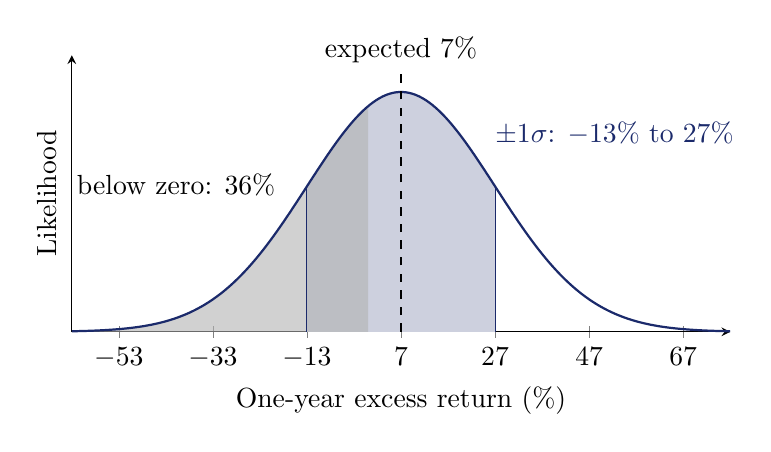
\begin{tikzpicture}[
    % One-year excess return ~ Normal(mean 7%, s.d. 20%)
    declare function={
      mu = 7; sd = 20;
      pdf(\x) = exp(-0.5*((\x-mu)/sd)^2)/(sd*sqrt(2*pi));
    }]
  \begin{axis}[
    width=0.82\linewidth, height=0.42\linewidth,
    axis lines=left,
    axis line style={-stealth, thin},
    xmin=-63, xmax=77, ymin=0, ymax=0.023,
    xtick={-53,-33,-13,7,27,47,67},
    ytick=\empty,
    xlabel={One-year excess return (\%)},
    ylabel={Likelihood},
    samples=200, domain=-63:77,
    clip=false,
  ]
    \addplot[name path=dens, draw=none] {pdf(x)};
    \path[name path=base] (axis cs:-63,0) -- (axis cs:77,0);

    % Plus or minus one standard deviation: -13% to 27%
    \addplot[fill=fenavy!22, draw=none]
      fill between[of=dens and base, soft clip={domain=-13:27}];
    % Below zero
    \addplot[fill=gray!60, fill opacity=0.6, draw=none]
      fill between[of=dens and base, soft clip={domain=-63:0}];

    % Edges of the one-sigma band
    \draw[fenavy] (axis cs:-13,0) -- (axis cs:-13,{pdf(-13)});
    \draw[fenavy] (axis cs:27,0)  -- (axis cs:27,{pdf(27)});

    % Density curve on top
    \addplot[fenavy, thick] {pdf(x)};

    % Expected return
    \draw[thick, dashed] (axis cs:7,0) -- (axis cs:7,0.0215)
      node[above] {expected 7\%};

    % Labels
    \node[anchor=west] at (axis cs:-64,0.0122) {below zero: 36\%};
    \node[fenavy, anchor=west] at (axis cs:25,0.0165)
      {$\pm 1\sigma$: $-13\%$ to $27\%$};
  \end{axis}
  \end{tikzpicture}
  \caption{One-year excess return on stocks, with an expected value of 7\% and
    a standard deviation of 20\%.}% <- replace with your caption
  \label{fig:07-oneyear}% <- replace with your label
\end{figure}


%\begin{figure}[htbp]
%\centering
%\includegraphics[width=0.85\linewidth]{images/fig01-1-one-year-return.png}
%\caption{One year's excess return on the stock market, assuming an expected excess return of 7\% and volatility of 20\%. The blue band covers the middle two-thirds of years, from $-13$\% to 27\%; the gray area is the 36\% of years with a negative excess return.}
%\label{fig:01-oneyear}
%\end{figure}


\textbf{The Sharpe ratio.} Sharpe (1966) proposed judging an investment by its excess return per unit of risk:
\begin{equation}
  \mathrm{SR} = \frac{E[R] - r_f}{\sigma}
  \label{eq:01-sr}
\end{equation}

The stock market's long-run Sharpe ratio is around 0.3 to 0.4 a year. Because leverage scales excess return and volatility equally, the Sharpe ratio does not change when a portfolio is levered up or down, which makes it the natural measure for comparing strategies (Figure~\ref{fig:01-sharpe-slope}).

\begin{figure}[htbp]
\centering
\includegraphics[width=0.85\linewidth]{images/fig01-2-sharpe-slope.png}
\caption{The Sharpe ratio is the slope of a line from the risk-free rate. Leverage moves a portfolio along its line, raising or lowering both excess return and volatility, but does not change the slope. A better strategy lies on a steeper line.}
\label{fig:01-sharpe-slope}
\end{figure}


\textbf{Risk, luck and skill.} Investors who make money in the stock market can do so for three different reasons. The distinction runs through the whole book.


\begin{itemize}
  \item \textbf{Bearing risk.} Stocks are riskier than Treasury bills, so over
  time they have paid more: this extra return is the equity premium defined
  above. An investor who simply buys and holds an index fund earns it without
  any special ability. Profit from bearing risk is a reward for risk, not
  evidence of skill.

  \emph{Examples.} (i) A retiree who has held an S\&P~500 index fund since
  1990 has earned far more than a savings account would have paid, without
  ever picking a stock. (ii) A manager who borrows to hold the index at
  1.5 times exposure beats the index in most years, but only because he
  carries 1.5 times its risk; in a crash he loses 1.5 times as much.
  (iii) A trader who sells out-of-the-money put options collects a small,
  steady premium month after month and looks like a genius, until a market
  crash wipes out years of gains. In each case the extra return is payment
  for risk that anyone could have taken.

  \item \textbf{Luck.} Returns are noisy, so some investors do well by
  chance, sometimes for years at a time. We also hear more about the winners
  than the losers, which makes luck look more common than it is.

  \emph{Examples.} (i) Ten thousand people each flip a coin every year to
  decide whether to hold stocks or cash. After ten years, about ten of them
  will have called the market right every single year, and some will write
  books about their method. (ii) A newsletter sends 1{,}000 readers a
  ``buy'' call on a stock and another 1{,}000 a ``sell'' call. Whichever way
  the stock moves, half the readers now hold a correct prediction, and the
  trick can be repeated on that half. (iii) An investor puts her savings into
  one small biotech company just before it receives surprise drug approval.
  The outcome was real; the evidence of ability is one draw.

  \item \textbf{Skill.} It is the ability to earn more than the
  risk taken explains: a return that a simple, cheap alternative carrying the
  same risk would not have delivered. Skill comes from better information,
  better analysis or better execution.

  \emph{Examples.} (i) \emph{Better information:} an analyst counts cars in
  retailers' parking lots from satellite images and forecasts sales before
  the companies report them. (ii) \emph{Better analysis:} a fund beats a
  portfolio with the same market, size and value exposures, after fees, over
  twenty years and across many independent bets. (iii) \emph{Better
  execution:} a trading firm buys and sells the same stocks as everyone else
  but pays less in trading costs and price impact, keeping a few basis points
  per trade that others give away.
\end{itemize}

\noindent\textbf{Exercise: which one is it?} Suppose an investor
consistently chooses the right stock at the right time. Before calling this
skill, ask two questions. First, \emph{does the risk explain it?} If the
investor's picks are mostly high-risk stocks bought during a rising market,
a cheap fund holding equally risky stocks might have done just as well, and
the profit is a reward for risk. Second, \emph{does luck explain it?} If the
record is short, or the investor is one of many whose picks we never hear
about, a run of good calls is what chance alone would produce. Only when the
answer to both questions is no does skill become the likely explanation. The
rest of this section shows how finance measures it.

Finance measures skill with \textbf{alpha}. Regress a strategy's excess return on the market's excess return:
\begin{equation}
  R_s - r_f = \alpha + \beta\,(R_m - r_f) + \varepsilon \nonumber
\end{equation}
where $R_s$ is the strategy's return, $R_m$ the market's return and $\varepsilon$ the part of the return the regression does not explain. The coefficient $\beta$ (\textbf{beta}) measures how much market risk the strategy carries, so $\beta\,(R_m - r_f)$ is the return that market exposure alone would have delivered. The intercept $\alpha$ is what is left over: the average return beyond what the strategy's market risk explains. For example, suppose a strategy has a beta of 0.6 and earns an average excess return of 6\% a year while the market earns 8\%. Market risk explains $0.6 \times 8 = 4.8$\%, so the strategy's alpha is $6 - 4.8 = 1.2$\% a year. Chapter 3 develops this regression and its extensions to other sources of risk.

A positive alpha is necessary for skill but not sufficient, because luck also produces positive alphas. Telling the two apart is the central problem of this chapter.

\textbf{Estimating a mean, and how uncertain the estimate is.} Given $T$ observations of a return with standard deviation $\sigma$, the sample mean has a \textbf{standard error} of $\sigma/\sqrt{T}$. The \textbf{t-statistic} of a mean is the estimate divided by its standard error; under the hypothesis that the true mean is zero, it has approximately a standard normal distribution, so values beyond about $\pm 1.96$ occur by chance only 5\% of the time. Applied to the Sharpe ratio, the same arithmetic gives a useful rule: the t-statistic of a strategy's mean return is approximately its annual Sharpe ratio times the square root of the number of years. A Sharpe ratio of 0.5 needs about 15 years of data to reach $t = 1.96$ (Figure~\ref{fig:01-years}).

\begin{figure}[htbp]
\centering
\includegraphics[width=0.85\linewidth]{images/fig01-3-years-needed.png}
\caption{How many years of return data are needed before a strategy's track record becomes statistically significant. The years count the length of the history being analyzed, not how long the strategy must trade or hold its positions. With a true Sharpe ratio of 0.5, about 15 years of data are needed to reach $t = 1.96$; with 0.25, about 61.}
\label{fig:01-years}
\end{figure}


\textbf{Worked example.} A strategy earns an average excess return of 0.5\% a month with a monthly standard deviation of 4\% over 10 years. Its annual mean is 6\%, its annual volatility 4\% $\times \sqrt{12} \approx 13.9$\%, and its Sharpe ratio $6/13.9 \approx 0.43$. The t-statistic is $0.5 / (4/\sqrt{120}) \approx 1.37$, not significant at 5\%, even though the strategy may be genuinely good.

\textbf{Further reading.} Bodie, Kane and Marcus, \emph{Investments}, chapters on risk, return and the historical record; Campbell, Lo and MacKinlay, \emph{The Econometrics of Financial Markets}, chapter 1 on returns; Cochrane, \emph{Asset Pricing}, for the theory of why expected returns differ.


\section{Efficient markets and the random walk}
\label{sec:01-efficient-markets}

The starting point for any claim about beating the market is the efficient market hypothesis. In Eugene Fama's (1970) formulation, a market is efficient if prices fully reflect available information. The intuition is competitive: if a predictable profit existed, traders would act on it, and their trading would push prices until the profit disappeared.

Fama distinguished three versions by the information set:

\begin{center}
\small
\begin{tabularx}{0.9\linewidth}{@{}>{\raggedright\arraybackslash}p{0.180\linewidth}>{\raggedright\arraybackslash}p{0.234\linewidth}>{\raggedright\arraybackslash}X@{}}
\toprule
Version & Prices reflect & Implication if true \\
\midrule
Weak form & Past prices and trading volume & Technical trading rules cannot earn abnormal returns \\
Semi-strong form & All public information & Analysis of public news and accounting data cannot earn abnormal returns \\
Strong form & All information, including private & Even insiders cannot earn abnormal returns \\
\bottomrule
\end{tabularx}
\end{center}

Few economists believe the strong form, and insider-trading laws exist because it fails. The weak and semi-strong forms are where the empirical debate happens, and where most claims in this book live.

\textbf{What efficiency does not imply.} Efficiency is often misread, so three clarifications matter:

\begin{enumerate}
  \item \textbf{It does not mean returns are unpredictable in every sense.} Expected returns can vary over time or across stocks as compensation for risk. A predictable return that is fair payment for risk is consistent with efficiency; a predictable return that is a free lunch is not. Separating the two is the joint-hypothesis problem: every test of efficiency is also a test of a model of what returns \emph{should} be.
  \item \textbf{It does not mean prices are always right.} It means mispricings are hard to identify and profit from after costs. Grossman and Stiglitz (1980) showed that a perfectly efficient market is impossible: if prices reflected everything, no one would pay to gather information. Markets must be inefficient enough to reward the people who make them efficient.
  \item \textbf{It does not mean volatility is unpredictable.} As Chapter 11 shows, risk is far more predictable than return.
\end{enumerate}

\textbf{The random walk as a benchmark.} If prices respond only to new, unpredictable information, price changes should look approximately like a random walk: tomorrow's change is unrelated to today's. Samuelson (1965) showed that properly anticipated prices fluctuate randomly. Lo and MacKinlay (1988) later rejected a strict random walk for weekly U.S. returns, so the model is not literally true. But it remains the right benchmark: any strategy must beat what a random walk, or a simple buy-and-hold position, would deliver.

For this book, the practical lesson is a prior. Before seeing evidence, a claim that a simple rule beats the market should be treated as unlikely. Not impossible, since the following chapters find some that survive, but unlikely enough to demand strong evidence.

\section{Signal and noise}
\label{sec:01-signal-noise}

The deeper reason claims are hard to verify is statistical: in finance, the signal is small and the noise is large. The differences between good and bad strategies are a few percent a year in expected return, while their returns move by fifteen or twenty percent a year at random.

\textbf{The Sharpe ratio, again.} The yardstick for a strategy is the Sharpe ratio of Equation~\eqref{eq:01-sr}. In this section we write $\mu$ for the strategy's expected return $E[R]$, so that $\mathrm{SR} = (\mu - r_f)/\sigma$, with all quantities annualized. Against the stock market's long-run Sharpe ratio of 0.3 to 0.4 (Section~\ref{sec:01-foundations}), a strategy with a true Sharpe ratio of 0.5 after costs would be a valuable discovery, and 1.0 would be exceptional.

\textbf{How precisely can we measure it?} With $T$ years of independent returns, the t-statistic for testing whether the true Sharpe ratio is zero is approximately
\begin{equation}
  t \approx \mathrm{SR}\,\sqrt{T}
  \label{eq:01-t}
\end{equation}
Equation~\eqref{eq:01-t} follows from the definition of the Sharpe ratio in Equation~\eqref{eq:01-sr} in four steps.

\begin{enumerate}
  \item \textbf{Estimate the mean.} Take $T$ years of annual excess returns. Their sample average, $\bar{x}$, is our estimate of the expected excess return $\mu - r_f$.
  \item \textbf{Find its standard error.} If the yearly returns are independent with volatility $\sigma$, the standard error of an average of $T$ of them is
  \begin{equation}
    \mathrm{SE}(\bar{x}) = \frac{\sigma}{\sqrt{T}} \nonumber
  \end{equation}
  \item \textbf{Form the t-statistic.} To test whether the true mean is zero, divide the estimate by its standard error:
  \begin{equation}
    t = \frac{\bar{x}}{\sigma/\sqrt{T}} = \frac{\bar{x}}{\sigma}\,\sqrt{T} \nonumber
  \end{equation}
  \item \textbf{Recognize the Sharpe ratio.} The ratio $\bar{x}/\sigma$ is the measured Sharpe ratio. Replacing $\bar{x}$ with the true mean $\mu - r_f$ gives the t-statistic we should expect on average:
  \begin{equation}
    t \approx \frac{\mu - r_f}{\sigma}\,\sqrt{T} = \mathrm{SR}\,\sqrt{T} \nonumber
  \end{equation}
  The result is approximate for two reasons: the measured mean differs from the true one, and in practice $\sigma$ must be estimated as well.
\end{enumerate}

The answer is the same with monthly or daily data. Sampling $k$ times a year gives $kT$ observations, each with mean $(\mu - r_f)/k$ and volatility $\sigma/\sqrt{k}$, so
\begin{equation}
  t = \frac{(\mu - r_f)/k}{(\sigma/\sqrt{k})/\sqrt{kT}} = \frac{\mu - r_f}{\sigma}\,\sqrt{T} \nonumber
\end{equation}
and the sampling frequency $k$ cancels.

By the same reasoning, the standard error of an estimated annual Sharpe ratio is roughly $1/\sqrt{T}$. Lo (2002) gives the refinements for non-normal and autocorrelated returns; the rough version is enough to see the problem. Setting $t = 1.96$, the usual 5\% significance threshold, in Equation~\eqref{eq:01-t} and solving for $T$ gives the number of years needed before a strategy's record can be distinguished from luck. Dividing both sides by SR gives $\sqrt{T} \approx 1.96/\mathrm{SR}$, and squaring gives
\begin{equation}
  T \approx \left(\frac{1.96}{\mathrm{SR}}\right)^2
  \label{eq:01-T}
\end{equation}

\begin{center}
\small
\begin{tabular}{@{}ll@{}}
\toprule
True Sharpe ratio & Years of data needed for $t = 1.96$ \\
\midrule
0.25 & 61 \\
0.50 & 15 \\
0.75 & 7 \\
1.00 & 4 \\
1.50 & 2 \\
\bottomrule
\end{tabular}
\end{center}

A strategy as good as the stock market itself needs more than two decades of data before its record is statistically convincing. Most fund track records, and most backtests shown to investors, are far shorter.

\textbf{Does the return frequency matter?} For the years-needed table above, no. Daily data give 252 observations a year instead of 12, but each daily return carries proportionally less information about the mean, so the years needed are the same. Table~\ref{tab:01-frequency} shows this for one strategy, with an expected excess return of 10\% a year, volatility of 20\% and so a Sharpe ratio of 0.5, observed over the same 16 years at three frequencies. The t-statistic is always the Sharpe ratio \emph{per period} times the square root of the \emph{number of periods}. Sampling more often multiplies the number of observations, but shrinks the Sharpe ratio of each one by the square root of that factor, and the two effects cancel.

\begin{table}[htbp]
\centering
\small
\caption{The same 16-year record measured annually, monthly and daily. Expected excess return 10\% and volatility 20\% a year, so the annual Sharpe ratio is 0.5. Daily figures assume 252 trading days a year.}
\label{tab:01-frequency}
\begin{tabular}{@{}lrrrrrr@{}}
\toprule
Frequency & Observations & Mean per & Volatility per & Sharpe ratio & $\sqrt{N}$ & $t$ \\
 & $N$ & period (\%) & period (\%) & per period & & \\
\midrule
Annual  & 16    & 10.000 & 20.00 & 0.500  & 4.00  & 2.00 \\
Monthly & 192   & 0.833  & 5.77  & 0.144  & 13.86 & 2.00 \\
Daily   & 4{,}032 & 0.040 & 1.26  & 0.0315 & 63.50 & 2.00 \\
\bottomrule
\end{tabular}
\end{table}

Going from annual to monthly data gives 12 times as many observations, but each has a mean 12 times smaller and a volatility $\sqrt{12}$ times smaller, so its Sharpe ratio is $\sqrt{12}$ times smaller. Since $\sqrt{N}$ grows by exactly $\sqrt{12}$, the t-statistic does not change. The same happens with 252 in place of 12 for daily data. This is why Equation~\eqref{eq:01-t} can be stated in years: $T$ is the number of observations only when the Sharpe ratio is measured over the same period, and for an annual Sharpe ratio that period is a year. Merton (1980) made this point: the precision of an estimated expected return depends on the length of the history, not on the sampling frequency. With log returns the reason is especially plain. The average annual log return over $T$ years depends only on the first and last prices,
\begin{equation}
  \bar{r} = \frac{\ln P_T - \ln P_0}{T}, \nonumber
\end{equation}
because every price in between is added once and subtracted once. Dividing a century into days rather than months adds no information about the mean, and its standard error stays at about $20/\sqrt{100} = 2$\%, as in Section~\ref{sec:01-foundations}. The same holds for every claim about \emph{average} returns, such as the equity premium, value, momentum and published anomalies, which is why Chapters 7 to 10 can test them on monthly data without losing anything.

Claims about \emph{risk} are different. Each additional observation adds information about how much returns vary, so the precision of an estimated volatility grows with the number of returns $N$, not just the number of years:
\begin{equation}
  \mathrm{SE}(\hat{\sigma}) \approx \frac{\sigma}{\sqrt{2N}} \nonumber
\end{equation}
With 20\% volatility and a century of data, the standard error is about 0.41 percentage points with monthly returns ($N = 1{,}200$) and about 0.09 with daily returns ($N \approx 25{,}200$), more than four times smaller. This is why the chapters on volatility (Chapter 11), value at risk (Chapter 13), delta hedging (Chapter 15) and trading costs (Chapter 6) use daily or even intraday data.

The rule ``the mean needs a long history, risk needs frequent data'' is a good guide, but it has limits.
\begin{itemize}
  \item \textbf{Very high frequency adds noise.} At intraday frequencies, the bounce between bid and ask prices and stale quotes distort measured returns, so for volatility, more frequent data help only up to a point.
  \item \textbf{Daily betas can be biased.} Stocks that trade infrequently react to market news with a delay, which makes their daily betas too low. Monthly data, or a correction that adds lagged market returns to the regression (Dimson, 1979), reduces the bias. This matters for the low-risk anomaly in Chapter 12.
  \item \textbf{Annualizing is not automatic.} The rules in Section~\ref{sec:01-foundations} for converting monthly figures to annual ones assume that returns are uncorrelated over time. When they are autocorrelated, as for many hedge funds and illiquid assets, a monthly Sharpe ratio multiplied by $\sqrt{12}$ can be badly off (Lo, 2002).
  \item \textbf{The cancellation is exact only for log returns.} For simple returns, the precision of the mean still depends mainly on the length of the history, but only approximately.
\end{itemize}

The practical lesson is to match the data to the claim. To measure an expected return more precisely, you need a longer history, not more frequent data; to measure risk, more frequent data help.

\textbf{What a ten-year record can tell you.} The ``10 years'' here is not how long the strategy holds its positions; the strategy may trade daily or monthly. It is the length of the track record you look at when you judge the strategy. A thought experiment shows how noisy that judgment is.

\begin{enumerate}
  \item \textbf{The strategy is genuinely good.} Suppose its true Sharpe ratio is 0.5. Nobody can see this number directly; we see only the Sharpe ratio measured from its realized returns.
  \item \textbf{The measurement is noisy.} With a 10-year record, the standard error of the measured Sharpe ratio is about $1/\sqrt{10} \approx 0.32$.
  \item \textbf{The record could show almost anything.} A 95\% range for the measured Sharpe ratio is $0.5 \pm 1.96 \times 0.32$, or about $-0.1$ to 1.1. Imagine watching the same strategy over many different decades. In one decade it looks like a star, with a Sharpe ratio near 1.0; in another it looks like a failure, near zero. The strategy is the same; only the decade differs.
  \item \textbf{Luck can look like skill.} A strategy with no skill has a true Sharpe ratio of zero, yet its measured Sharpe ratio exceeds 0.5 whenever the noise is more than $0.5/0.32 \approx 1.6$ standard errors. That happens in roughly 6\% of decades, by luck alone.
\end{enumerate}

Figure~\ref{fig:01-ten-year} draws the two cases side by side. The curves overlap heavily: a measured Sharpe ratio of 0.4, for example, is quite consistent with both a genuinely good strategy and a useless one. A ten-year record cannot reliably tell them apart.

\begin{figure}[htbp]
\centering
\includegraphics[width=0.85\linewidth]{images/fig01-4-ten-year-record.png}
\caption{What a 10-year record can show. The gray curve is the range of Sharpe ratios a strategy with no skill produces over different decades; the blue curve is the same for a strategy with a true Sharpe ratio of 0.5. The shaded tail is the 6\% of decades in which the useless strategy beats 0.5 by luck.}
\label{fig:01-ten-year}
\end{figure}

\textbf{Why prediction is harder than it looks.} The same arithmetic applies to forecasting. A model that explains just 1\% of the variation in monthly returns would be worth a great deal to an investor (Campbell and Thompson 2008 make this point). But an $R^2$ of 1\% is almost impossible to distinguish from zero in a few decades of data, and almost trivially easy to produce by accident when many models are tried. Small true effects, large noise and short samples together make finance a field where false discoveries are easy and true ones are hard to confirm.

\section{Cautions: Why backtests can mislead}
\label{sec:01-backtests}

A backtest applies a strategy's rules to historical data to show how it would have performed. It is the most common evidence offered for a strategy and the easiest to get wrong. Seven problems account for most misleading backtests; later chapters treat each in depth.

\begin{enumerate}
  \item \textbf{Selection across many trials.} If you test 100 rules and report the best, its record overstates what it will deliver. This is the subject of the lab, and of Chapter 4.
  \item \textbf{Overfitting parameters.} Tuning a rule's settings (a 47-day average instead of 50, a threshold of 1.3 instead of 1.5) fits the noise in the sample. Each added parameter is another hidden trial.
  \item \textbf{Look-ahead bias.} Using information that was not available at the time, such as revised economic data or accounting figures before their release date (Chapter 2).
  \item \textbf{Survivorship bias.} Testing only on companies or funds that still exist, which excludes the failures (Chapter 2).
  \item \textbf{Ignoring costs.} Spreads, commissions, market impact, borrowing fees and taxes can erase a paper profit, especially for high-turnover strategies (Chapter 6).
  \item \textbf{Short or unrepresentative samples.} A decade of data may contain only one market regime. As Section~\ref{sec:01-signal-noise} showed, a short sample cannot separate skill from luck.
  \item \textbf{A story told after the fact.} Once a pattern is found, a plausible explanation is easy to write. The story makes the result feel robust, but it was written to fit the data, not tested against it.
\end{enumerate}

These problems compound. A backtest can be honest in every visible detail, using correct prices, real costs and no look-ahead, and still mislead because it is the best of many attempts that are never shown.

\begin{callout}
\textbf{What Failed: butter in Bangladesh.} To show how easy data mining is, David Leinweber searched a United Nations database for series that tracked the S\&P 500. Butter production in Bangladesh fit well; adding U.S. cheese production and the sheep population of Bangladesh and the United States raised the fit further, with an $R^2$ that looked like a breakthrough. The relationship, of course, predicted nothing afterward. The example was a joke with a serious point: search enough series, and a near-perfect fit is guaranteed. Leinweber later wrote it up as ``Stupid Data Miner Tricks'' (2007).
\end{callout}

\section{The claims-on-trial method and the verdict scale}
\label{sec:01-method}

Every claim chapter and every lab opens with a line labelled \textbf{Claim on trial}. The label is a reminder of who does the work: you are not told whether the claim is true, you test it. The book's subtitle, \emph{Active Learning by Verifying Famous Claims}, describes the bargain. Each trial needs a method (a regression, a backtest, a volatility model, a hedge), and you learn that method in order to reach a verdict, then use it again in later trials until it is second nature.

The rest of this book applies one method to every claim. It is simple enough to remember and strict enough to protect against the problems in Section~\ref{sec:01-backtests}.

\begin{enumerate}
  \item \textbf{Claim} --- State what is asserted in one testable sentence. ``Momentum works'' is vague; ``stocks with the highest 12-month returns, skipping the last month, outperform the lowest by a positive average return after costs'' can be tested.
  \item \textbf{Understand} --- Learn how the idea works and how the original evidence was produced: the data, sample period, method and number of alternatives the authors tried.
  \item \textbf{Verify} --- Rebuild the result yourself, then stress-test it: out of sample, in other markets, after costs, after publication.
  \item \textbf{Judge} --- Reach a verdict on the scale below, dated with the sample period tested.
  \item \textbf{Apply} --- State what an investor or practitioner can actually use, and what remains open.
\end{enumerate}

\textbf{The verdict scale}

\begin{center}
\small
\begin{tabularx}{0.9\linewidth}{@{}>{\raggedright\arraybackslash}p{0.162\linewidth}>{\raggedright\arraybackslash}X@{}}
\toprule
Verdict & Meaning \\
\midrule
Survives & The result replicates, holds out of sample and in other markets, and remains economically meaningful after costs. \\
Weakens & The result is real but smaller, less reliable, or narrower than claimed, for example only in small stocks or before publication. \\
Fails & The result does not replicate, or disappears out of sample or after costs. \\
Provisional & The evidence is too new or too mixed for a firm verdict. \\
\bottomrule
\end{tabularx}
\end{center}

Two habits make the method work. First, \textbf{decide the test before seeing the result}: write down the claim, the data and the pass criteria first, so the test cannot be bent to fit the outcome. Second, \textbf{always ask ``compared to what?''}: every claim is judged against a simple benchmark, such as the market, the historical average or a naive rule, never against zero.

This chapter's lab applies the method to a claim at the root of the whole field: whether a track record can reveal real skill.

\section{Lab 1: Brilliant by chance}
\label{sec:01-lab}

\begin{callout}
\textbf{Lab 1 at a glance.} Claim on trial: a long enough track record can reveal real skill. Data: monthly U.S. market excess returns and Treasury bill rates since 1926, from the Kenneth R. French Data Library (downloaded automatically). Tools: Python with pandas, NumPy and matplotlib, plus the book's fintest module. Time: about one hour, including the guided notebook; the code itself runs in seconds. Code: repository folder \texttt{ch01-brilliant-by-chance/}.
\end{callout}

\subsection*{Design}

The lab answers the claim by first measuring what luck alone can do. It builds strategies whose skill we know for certain: none. Whatever these strategies achieve sets the bar that a real strategy's record must clear. Each of 1,000 strategies is, every month, either invested in the stock market or holding Treasury bills. It switches between the two at random, with an average holding period between 3 and 24 months, so the strategies look like real market-timing rules. They use no information at all, and each month's position is fixed before that month's return is known. The design follows the logic of Bailey, Borwein, L\'opez de Prado and Zhu (2014), who show that the best of many backtests can look impressive by chance alone, and of Harvey, Liu and Zhu (2016), who argue that the usual $t > 2$ hurdle is far too low when many strategies are tried.

The sample is split in two. The first half, roughly 1926 to 1975, plays the role of the \textbf{backtest}: the period in which a researcher would test the strategies and choose the best. The second half, roughly 1976 to today, is the period \textbf{after selection}: what an investor who adopted the chosen strategy would have experienced.

\textbf{Measuring skill.} A strategy that is in the market part of the time will earn part of the market's return with no skill at all. Skill is therefore measured as \textbf{alpha against buy-and-hold} (Section~\ref{sec:01-foundations}): the intercept in a regression of the strategy's excess return on the market's excess return. For every strategy in this lab, the true alpha is zero. Each alpha is tested with a t-statistic using Newey--West standard errors, which Chapter 3 explains.

\subsection*{Three parts}

\begin{enumerate}
  \item \textbf{Signal and noise.} Measure the market's Sharpe ratio over the full sample and over every 10-year window, and compute how many years are needed to detect a given Sharpe ratio (Figure 1.5 and the table in Section~\ref{sec:01-signal-noise}).
  \item \textbf{Brilliant by chance.} Backtest the 1,000 random strategies, count how many look significant, pick the best, and follow all of them into the period after selection (Figures 1.6 to 1.8).
  \item \textbf{The cost of searching.} Show how the best backtest t-statistic rises as more strategies are tried, from 1 to 1,000 (Figure 1.9).
\end{enumerate}

\subsection*{What theory predicts}

Because every strategy has zero skill, statistics tells us in advance roughly what to expect, which makes the lab a test of your intuition:

\begin{center}
\small
\begin{tabularx}{0.9\linewidth}{@{}>{\raggedright\arraybackslash}p{0.450\linewidth}>{\raggedright\arraybackslash}X@{}}
\toprule
Measure & Expected for 1,000 zero-skill strategies \\
\midrule
Strategies passing $t > 1.96$ in the backtest & About 25 (2.5\%), typically between about 15 and 50 \\
Best backtest t-statistic & About 3.2 \\
Threshold that controls false discoveries across all 1,000 (Bonferroni, 5\%) & $t > 3.89$ \\
Correlation between backtest and later t-statistics & About zero \\
Average later t-statistic of the backtest ``winners'' & About zero \\
\bottomrule
\end{tabularx}
\end{center}

The count of significant strategies varies more than a simple coin-flip model suggests, for two reasons the lab asks readers to explain: all 1,000 strategies share one market history, and heavy-tailed returns make standard errors slightly too small.

\subsection*{What readers will see}

The chapter presents five exhibits. Figure 1.5 tracks the market's 10-year Sharpe ratio. Figure 1.6 shows the 1,000 backtest t-statistics against the bell curve that pure luck predicts. Figure 1.7 plots the growth of \$1 in the best random strategy against the market, with the backtest and after-selection periods marked. Figure 1.8 plots each strategy's backtest t-statistic against its later t-statistic. Figure 1.9 shows how the best backtest improves with the number of strategies tried.

\emph{[Draft note: the figures and numbers are generated by running the lab on the Kenneth French data at the time of publication. The book prints the real-data results; the text above does not anticipate them beyond what statistical theory predicts.]}

\subsection*{Your verdict}

The lab ends by asking readers to write their own verdict on the claim in two or three sentences, using their numbers. The expected conclusion is \textbf{survives, with conditions}. A track record can reveal real skill, but only when three conditions hold:

\begin{enumerate}
  \item \textbf{It is long enough for its Sharpe ratio.} About $(1.96/\mathrm{SR})^2$ years: roughly 15 for a Sharpe ratio of 0.5 and 4 for 1.0 (Section~\ref{sec:01-signal-noise}).
  \item \textbf{It clears a bar that allows for how many strategies were tried.} After 1,000 tries, that bar is $t > 3.89$, not 1.96; the random strategies in Parts 2 and 3 show why.
  \item \textbf{It keeps working on data that played no part in choosing it}, such as the period after selection.
\end{enumerate}

A record that meets all three is real evidence of skill. A short record, or the best of many tries judged by the usual bar, is not.

\textbf{What the verdict means for you.} Profits can come from bearing risk, from luck or from skill (Section~\ref{sec:01-foundations}), and skill can be found. The conditions above are not obstacles; they are the specification a credible strategy must meet. Lab extension~9 lets you plant a genuinely skilled strategy among the 1,000 and see what it takes for it to stand out. The rest of the book gives you the tools to meet each condition, and later chapters find strategies whose alpha survives testing.

\section{What investors can use}
\label{sec:01-investors}

The practical lesson of this chapter is to judge evidence by \textbf{how it was produced}, not by how good it looks. A spectacular track record and a modest one can carry the same information, or none, depending on the search behind them. The same lesson tells you what a convincing record looks like: long enough for its Sharpe ratio, honest about the number of tries, and confirmed on new data.

\textbf{Rules of thumb}

\begin{enumerate}
  \item Treat any backtest as the best of many tries unless you are shown otherwise.
  \item Discount short records heavily. Under ten years, a record says little about skill, as Section~\ref{sec:01-signal-noise} showed.
  \item Prefer evidence from data that played no part in designing the strategy: the period after a paper's publication, after a fund's launch, or after a rule was fixed.
  \item Ask for the benchmark. A strategy's return means little until it is compared with what a simple alternative, such as an index fund, earned over the same period.
  \item Know what a convincing record needs: about 15 years for a Sharpe ratio of 0.5, a higher bar after a search, and results that hold after the strategy was fixed.
\end{enumerate}

\textbf{Questions to ask a fund manager or strategy vendor}

\begin{itemize}
  \item How many strategies or parameter settings did you test before choosing this one?
  \item Which part of this record is a live track record, and which part is a backtest?
  \item When was the strategy's design fixed, and how has it performed since then?
  \item What is the benchmark, and what is the strategy's alpha against it, with its t-statistic?
  \item What happened to the other strategies or funds you launched at the same time?
  \item Are transaction costs, fees and taxes included?
\end{itemize}

\section{Looking ahead}
\label{sec:01-ahead}

This chapter showed that prices are hard to predict, that the noise in returns hides real effects and manufactures false ones, and that selection turns luck into impressive backtests. The rest of the book builds on these points in three steps.

\textbf{Part I continues} with Chapter 2, on the data itself: how survivorship bias, look-ahead bias and micro-cap stocks inflate results before any statistics are run.

\textbf{Part II} turns the warnings of this chapter into tools: statistics built for noisy returns (Chapter 3), corrections for multiple testing such as the deflated Sharpe ratio (Chapter 4), honest out-of-sample design (Chapter 5) and transaction costs (Chapter 6).

\textbf{Parts III to VII} then put the field's most important claims on trial, from return predictability and the value premium to risk models, option hedging, bond, credit and currency markets, and machine learning. Each chapter ends with a verdict. Some claims survive. That is the point of the method: not to dismiss every finding, but to separate the ones that hold from the ones that only looked good.

\section*{Exercises}
\addcontentsline{toc}{section}{Exercises}

\subsection*{Conceptual (all readers)}

\begin{enumerate}
  \item Explain in your own words why a market in which prices fully reflected all information could not exist (Grossman and Stiglitz). What does this imply for anyone claiming to beat the market?
  \item A fund has returned 4\% a year more than its benchmark for five years, with a tracking error (volatility of the excess return) of 8\%. Compute the t-statistic of its excess return. Is the record evidence of skill?
  \item Using the formula in Section~\ref{sec:01-signal-noise}, how many years of data would you need to detect a strategy with a true Sharpe ratio of 0.3? What does your answer imply for most fund track records?
  \item A newsletter reports that its ``crash indicator'' correctly called the last three bear markets. List three questions you would ask before believing it.
  \item Pick a recent strategy, fund or AI-based product advertised online. Using the problems listed in Section~\ref{sec:01-backtests}, identify which ones could inflate its record, and write the first question you would ask.
\end{enumerate}

\subsection*{Lab extensions (technical readers)}

\begin{enumerate}
  \setcounter{enumi}{5}
  \item Re-run Lab 1 with five different seeds. Record the number of strategies with $t > 1.96$ and the best $t$ each time. How much do they vary, and why?
  \item Increase the number of strategies to 10,000. How large is the best backtest t-statistic? Compare it with Figure 1.9 and with the approximation $\sqrt{2 \ln N}$.
  \item Move the split between backtest and after-selection periods to 1990. Do the conclusions change?
  \item Add one ``needle'' strategy with genuine skill: in the market with probability 0.55 in months the market rises and 0.45 in months it falls. Where does it rank among the 1,000 in the backtest? What does that tell you about finding real skill among many tries?
  \item Replace the random strategies with 200 moving-average timing rules (different window lengths). Unlike the random strategies, these might contain real information. How would you decide whether the best rule's backtest shows skill? Write down your test before running it.
\end{enumerate}

\section*{References}
\addcontentsline{toc}{section}{References}

\begin{itemize}
  \item Bailey, D. H., Borwein, J. M., L\'opez de Prado, M. and Zhu, Q. J. (2014). Pseudo-Mathematics and Financial Charlatanism: The Effects of Backtest Overfitting on Out-of-Sample Performance. \emph{Notices of the American Mathematical Society} 61(5): 458--471.
  \item Campbell, J. Y. and Thompson, S. B. (2008). Predicting Excess Stock Returns Out of Sample: Can Anything Beat the Historical Average? \emph{Review of Financial Studies} 21(4): 1509--1531.
  \item Dimson, E. (1979). Risk Measurement When Shares Are Subject to Infrequent Trading. \emph{Journal of Financial Economics} 7(2): 197--226.
  \item Fama, E. F. (1970). Efficient Capital Markets: A Review of Theory and Empirical Work. \emph{Journal of Finance} 25(2): 383--417.
  \item Grossman, S. J. and Stiglitz, J. E. (1980). On the Impossibility of Informationally Efficient Markets. \emph{American Economic Review} 70(3): 393--408.
  \item Harvey, C. R., Liu, Y. and Zhu, H. (2016). \ldots and the Cross-Section of Expected Returns. \emph{Review of Financial Studies} 29(1): 5--68.
  \item Leinweber, D. J. (2007). Stupid Data Miner Tricks: Overfitting the S\&P 500. \emph{Journal of Investing} 16(1): 15--22.
  \item Lo, A. W. (2002). The Statistics of Sharpe Ratios. \emph{Financial Analysts Journal} 58(4): 36--52.
  \item Lo, A. W. and MacKinlay, A. C. (1988). Stock Market Prices Do Not Follow Random Walks: Evidence from a Simple Specification Test. \emph{Review of Financial Studies} 1(1): 41--66.
  \item Merton, R. C. (1980). On Estimating the Expected Return on the Market: An Exploratory Investigation. \emph{Journal of Financial Economics} 8(4): 323--361.
  \item Samuelson, P. A. (1965). Proof That Properly Anticipated Prices Fluctuate Randomly. \emph{Industrial Management Review} 6(2): 41--49.
  \item Sharpe, W. F. (1966). Mutual Fund Performance. \emph{Journal of Business} 39(1): 119--138.
\end{itemize}

\textbf{Data:} Kenneth R. French Data Library, Fama/French 3 Factors, monthly. \url{https://mba.tuck.dartmouth.edu/pages/faculty/ken.french/data_library.html}

\includepdf{infographic/ch01_infographic.pdf}
\input{chapters/ch02.tex}
\includepdf{infographic/ch02_infographic.pdf}

%--------------------------- PART II -----------------------------------%
%\addcontentsline{toc}{chapter}{PART II: ...}
\input{chapters/ch03.tex}
\includepdf{infographic/ch03_infographic.pdf}
\input{chapters/ch04.tex}
\includepdf{infographic/ch04_infographic.pdf}
\input{chapters/ch05.tex}
\input{chapters/ch06.tex}

%--------------------------- PART III ----------------------------------%
%\addcontentsline{toc}{chapter}{PART III: ...}
\input{chapters/ch07.tex}
%\input{chapters/ch08.tex}
%\input{chapters/ch09.tex}
%\input{chapters/ch10.tex}

%--------------------------- PART IV -----------------------------------%
%\input{chapters/ch11.tex}
%\input{chapters/ch12.tex}
%\input{chapters/ch13.tex}
%\input{chapters/ch14.tex}
%\input{chapters/ch15.tex}

%--------------------------- PART V ------------------------------------%
%\input{chapters/ch16.tex}
%\input{chapters/ch17.tex}
%\input{chapters/ch18.tex}

%--------------------------- PART VI -----------------------------------%
%\input{chapters/ch19.tex}
%\input{chapters/ch20.tex}

%--------------------------- PART VII ----------------------------------%
%\input{chapters/ch21.tex}
%\input{chapters/ch22.tex}
%\input{chapters/ch23.tex}

%--------------------------- PART VIII ---------------------------------%
%\input{chapters/ch24.tex}
%\input{chapters/ch25.tex}
%\input{chapters/ch26.tex}
\input{chapters/furtherreading.tex}

%--------------------------Keyword Page Index------------------------%
\backmatter
\clearpage
\printindex

\thispagestyle{empty}
\end{document}
